\setstretch{1.5}
\chapter{Introduction}

\tab Microelectronic devices are finding wide applications in many diverse areas of life; from
high-end engineering workstations to washing machines, integrated circuits are found everywhere. The desire to achieve better performance and more functionality has led to a
continuous increase in the device density on these chips. This has most often been accomplished by reducing the featme size of the individual devices. Commercial devices are
presently fabricated with feature sizes on the order of 0.35 /xm, while much smaller devices are under development in research laboratories. As critical dimensions shrink, better
process control becomes important for a number of the fabrication steps. Tighter process
control requirements will accelerate the adoption of in situ control methods and metrology
[96]. Reactive ion etching (RIE) is one area in which real-time process control will become
increasingly important [82].


\tab The focus of this dissertation is to explore how real-time feedback control may be used
to improve the reactive ion etching process. In particular, the goals of this research were
to 1) configure a plasma etch tool to allow real-time feedback control, 2) develop controloriented models of the etching process, 3) develop control algorithms based on these models,
and 4) show that the application of real-time feedback control can improve the quality of the etch process. In this introduction, I will provide a brief overview of microelectronic
fabrication processes. This will be followed by a detailed discussion of the reactive ion
etching process. The application of real-time control techniques to a variety of fabrication
processes will then be described. I will conclude with a brief outline of the chapters of this
dissertation.


\section{Microelectronic Fabrication}

\tab Integrated circuits are fabricated on thin (~ 0.5 mm) disks of crystalline silicon known
as wafers. These wafers are currently as large as 200 mm (8 inches) in diameter, and even
larger wafers are planned for the near future. Each wafer may contain as many as 100
integrated circuit chips, with each chip containing over 3 million devices. Each of these
devices needs to be uniformly fabricated with very small defect densities.

\tab The fabrication process is often broken down into a number of mask levels; there are
over twenty of these mask levels in the fabrication of a modern microprocessor. At each level
several unit process steps are performed. These steps can be loosely arranged into three
categories: film growth/deposition, doping, and pattern transfer. A complete description
of the unit process steps can be found in [66,101,108] and the integration of these steps to
fabricate working devices can be found in [101,107]. The etching process is part of pattern
transfer, so I will concentrate on describing this category.

\tab Pattern transfer can be broken down into two process steps. In a process known as
lithography, the desired geometric pattern is transfered from a mask to the mask layer
on the wafer surface. Then, during the etch process, material is removed from areas left
exposed by the mask layer. My research focused on applying real-time feedback control to
the latter of these steps.

\subsection{Lithography}
\tab The most commonly used material for the masking layer is a photosensitive polymer known as photoresist. Other materials (such as oxides, nitrides, and metals) are also used as masking layers, though photoresist is still used to define patterns in them. The lithographic process for photoresist is shown in Figure 1.1. First, the photoresist is spin-coated onto the wafer substrate and baked dry. The desired pattern for the mask level is then projected onto the photoresist. This is commonly done using ultraviolet light, though x-rays and electron beams are used in some applications. There are two types of photoresist, positive and negative. Positive photoresist contains an inhibitor component that prevents dissolution in a solvent [66]. During exposure, this inhibitor is chemically transformed and the resist becomes solnble. The resist is then developed using a solvent to dissolve the exposed regions. In the case of negative resist, the absorption of photons leads to crosslinking of the polymers [66]. During development, the crosslinked regions are not dissolved and the negative of the mask pattern is formed in the resist.

\subsection{Etching}
\tab After the pattern has been transferred to the mask layer, the material left unprotected by the mask is removed. This process is known as etching. My research focused on the etching of polycrystalline silicon (polysilicon).

\tab The etching process must be controlled to only remove the desired material layer, leaving the underlying layer essentially untouched. There are a number of characteristics that determine the quality of the etching process. These include, but are not limited to: Etch Rate The rate of removal of material.

\begin{figure}[H]
	\centering
	\bf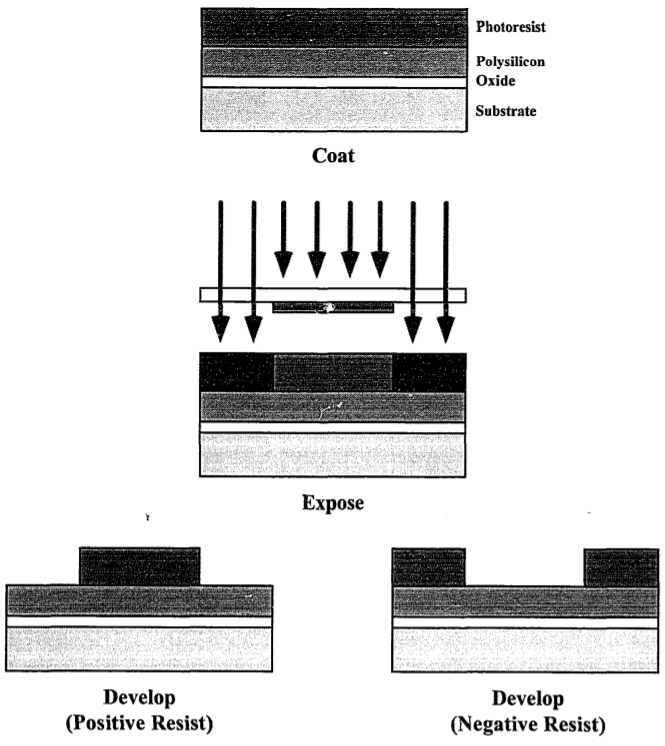
\includegraphics[scale = .75]{Figure 1.1}
	\caption{The lithographic process.}
	\label{fig:1.1}
\end{figure}

\begin{figure}[H]
	\centering
	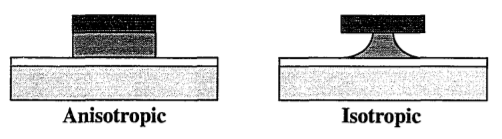
\includegraphics[scale = .75]{Figure 1.2}
	\bf\caption{Anisotropic and isotropic etching of small linewidths.}
	\label{fig:1.2}
\end{figure}

\noindent\textbf{Selectivity:} The etch rate ratio between the layer being etched and other \\
\indent layers, such as the photoresist or the underlying film.

\vspace{.25cm}

\noindent\textbf{Anisotropy:} The dependence of etch rate on direction. This usually refers to 
\indent greater
vertical than horizontal etch rate.

\vspace{.25cm}

\noindent\textbf{Uniformity:} The variation of the etch across the entire wafer or between\\ 
\indent multiple wafers in batch reactors.

\vspace{.25cm}

\noindent\textbf{Surface Damage:} Damage to the surface caused by the etch.

\vspace{.25cm}

A useful etch process has a number of requirements on these characteristics [108]. In order to achieve high throughput, the etch rate should be rapid. Additionally, in many recipes the etch time is predetermined; therefore, the etch rate needs to have little variation from run to run. In order to preserve the integrity of the masked pattern, the etch needs to be highly selective with respect to the masking layer; otherwise mask erosion will lead to changes in critical dimensions. Selectivity to the underlying layer is also necessary, as it is important not to remove a significant amount of material from this layer. This is especially important in the etching of polysilicon where the gate oxide below the polysilicon can be as thin as lOOÂor less. The etch needs to be highly uniform so that the same amount of material is removed across the entire wafer. The degree of anisotropy is important in order to achieve an acceptable sidewall profile. Sidewall profiles need to be vertical when etching 

\begin{figure}[H]
	\centering
	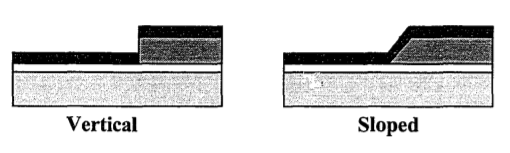
\includegraphics[scale = .75]{Figure 1.3}
	\bf\caption{Step coverage over vertical and sloped sidewalls.}
	\label{fig:1.3}
\end{figure}

\noindent small linewidths; otherwise there will be a loss in the integrity of the transfered pattern,as shown in Figure 1.2. However, as is shown in Figure 1.3, sloped sidewalls are necessary when step coverage by subsequent materials is required. Finally, the electrical properties of the material below that layer being etched must be undamaged.

One of the early techniques for removing materials is known as wet etching. In wet etching the wafers are dipped into a liquid solution, such as hydrofluoric acid (HF), which chemically reacts with the exposed surface. Through the appropriate choice of chemistry, it is possible to get very high selectivity to both the mask and underlying layer. However, wet etching is isotropic \footnote{There are situations where the orientation of the crystal can lead to an anisotropic wet etch, but these are beyond the scope of this introduction.}; i.e., material is physically removed in a direction normal to the surface. As depicted in Figure 1.2, when the critical dimensions are of the same size as the thickness of the layer being etched, isotropic etching can lead to significant changes in the desired linewidths. In this case, it is desirable to have a controlled degree of anisotropy in the etch.

As linewidths became smaller, an alternative technique known as dry etching emerged. In this technique, wafers are etched by being exposed to a low temperature plasma, as opposed to a liquid etchant. Dry etching can be broken down into a number of different regimes: plasma etching, sputter etching, and reactive ion etching. In plasma etching, neutral radicals generated in the plasma chemically react with the wafer surface to removematerial. This process tends to be highly isotropic in nature. In sputter etching (or a related technique known as ion milling \footnote{Ion milling is similar to sputter etching except that ions are not generated in a plasma but from an ion
	source in a high vacuum environment.}), material is physical removed by high energy ion bombardment [43]; this provides highly anisotropic etching but unacceptable selectivities and surface damage. In between these two extremes is reactive ion etching, where the etch is both chemical and physical in nature. By the appropriate choice of conditions, tradeoffs between anisotropy, selectivity, and surface damage can be made. Today, reactive ion etching is the main etch process used in integrated circuit production.


\section{Reactive Ion Etching}

\tab In reactive ion etching, material is removed through the interaction of neutral radicals and ions from the plasma with the wafer surface. In this section, I will first present an overview of the plasmas used for reactive ion etching. This will be followed by a discussion of the various etch mechanisms.

\subsection{Plasma Properties}

\tab A plasma is a collection of free charged particles moving in random directions; on average a plasma is electrically neutral and thus exhibits no net charge [68]. Plasmas used for semiconductor fabrication are, in general, weakly ionized, electrically driven, and not in thermal equilibrium. Overviews of plasmas used for microelectronic processing can be found in [16,45,68,108].

In reactive ion etching, the plasmas are generated in a vacuum chamber at pressures between 5 and 100 mTorr. A typical parallel plate reactive ion etcher is shown in Figure 1.4. A
mixture of gases enters the chamber through a showerhead in the upper electrode. Chamber pressure is controlled by a throttle

\begin{figure}[H]
	\centering
	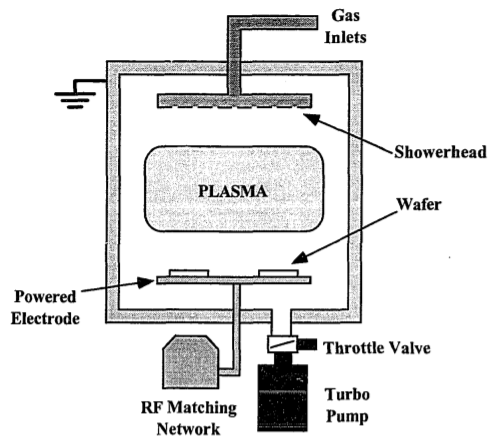
\includegraphics[scale = .75]{Figure 1.4}
	\bf\caption{Typical parallel plate reactive ion etcher}
	\label{fig:1.4}
\end{figure}

\noindent or sliding valve which regulates the exhaust of process gases by a high vacuum pump. A high frequency \footnote{Typically 13.56 MHz, a frequency which has been allotted by the Federal Communications Commission for industrial, scientific, and medical use [101].} rf generator is capacitively coupled to the lower electrode, while the showerhead and chamber walls are grounded. The application of
a large electric field across the electrodes results in ionization of the feed gas and generation of the plasma.


The electric field causes free electrons in the chamber to accelerate to high energies (~ 2eV) and these electrons collide with various species in the gas, thereby inducing a number of reactions. The most important of these collisions in sustaining the plasma is electron impact ionization in which the primary electron removes an electron from the atom, producing a positive ion and two electrons [16]. These two electrons are accelerated by the field and produce additional collisions, often causing more ionizations. It is this chain reaction that sustains the plasma. If the colliding electron does not have sufficient energy to ionize the atom, it still may excite a bound electron to a higher energy level. When this electron relaxes down to a lower energy state, the atom emits a photon. It is this process that gives a plasma its characteristic glow and why plasmas are often referred to as glow discharges. Electrons may also collide with molecules and break the bonds between atoms. This dissociation process results in atoms and molecules, both neutral and ionized. Typically, on the order of 10\% of the feed gas is dissociated [42]. Even with all of these
various collision processes, the ionization for plasmas used in RIE is typically between 10\textsuperscript{-6} and 10\textsuperscript{-4}; hence, these plasmas are made up mostly of neutral molecules.

The feed gas mixture used to produce the plasma depends on the material being etched. The chemistries used to etch various materials are shown in Table 1.1. In this research,
real-time control was applied to CF4 and CF4/O 2 etching of polysilicon. A large number of reactions occur in these plasmas; many of which are listed in [12,27]. The dominant
reactions include [91]


\begin{align}
	e^{-} + \text{CF}_{4} &\rightarrow \text{CF}^{+}_{4} + \text{F} + 2e^{-},\\
	e^{-} + \text{CF}_{4} &\rightarrow \text{CF}_{4} + 2\text{F} + 2e^{-},\\
	\text{CF}_{3} + \text{CF}_{3} &\rightarrow \text{C}_{2}\text{F}_{6},\\
	\text{CF}_{3}+\text{F} &\rightarrow \text{CF}_{4},\\
	\text{CF}_{2}+2\text{F} &\rightarrow \text{CF}_{4}.
\end{align}

The acceleration of the electrons by the rf field not only causes dissociation and ionization of the gas species, but also induces a bias on the electrode. This can be seen by assuming that the plasma potential is near zero, with respect to ground, and considering the model of

\begin{table}[H]
	\centering
	\begin{tabular}{|c|c|}
		\hline
		Material & Plasma Chemistries \\
		\hline
		Si & $\text{CF}_{4} $, $\text{CF}_{4}$/$\text{O}_{2} , \text{CI}_{2}, \text{SF}_{6}/\text{O}_{2}/\text{CI}_{2}, \text{NF}_{3}, \text{CCI}_{4}, \text{Br}_{2}$ \\
		\hline
		$\text{SiO}_{2}$ & $\text{CF}_{4}, \text{CF}_{4}/\text{H}_{2}, \text{CHF}_{3}\text{O}_{2}$ \\
		\hline
		$\text{SiN}_{3}$ & $\text{CF}_{4}/\text{O}_{2}/\text{H}_{2}, \text{CHF}_{3}$ \\
		\hline
		Silicides & $\text{O}_{2}, \text{CF}_{4}/\text{O}_{2}, \text{SF}_{6}/\text{O}_{2}$\\
		\hline
		Al & $\text{BCI}_{3}, \text{BCI}_{3}/\text{CI}_{2}, \text{CCI}_{4}/\text{CI}_{2}/\text{BCI}_{3}, \text{SiCl}_{4}/\text{Cl}_{2}$ \\
		\hline
	\end{tabular}
	\bf\caption{ Etch chemistries.}
	\label{table:1.1}
\end{table}

\noindent the rf discharge circuit shown in Figure 1.5. In this figure, $\text{V}_{a}$ is the voltage of the generator, $\text{V}_{b}$ is the voltage of the powered electrode, $\text{V}_{1}$ is the potential between the plasma and the powered electrode, $\text{V}_{2}$ is the potential between the plasma and the grounded electrode, and $\text{A}_{1}$ and $\text{A}_{2}$ are the surface areas of the powered and grounded electrodes, respectively. In order to sustain the discharge, ion current to the electrode must balance the electron current. Because the electrons are much lighter than the ions ($m_{e} \approx 10^{-4}m_{i}$), they require a much smaller field to conduct a given current. In order to balance the electron and ion fluxes, a negative dc bias develops on the powered electrode [52]. Therefore, as shown in Figure 1.6, $\text{V}_{b}$ is positive for only a small portion of the rf cycle. The thickness across which this dc voltage develops is known as the sheath. The presence of the bias voltage leads to almost continuous bombardment of the wafer by the ions. At the same time, due to their small mass, electrons are rapidly accelerated away from the electrode. Therefore, the electron density in the sheath is drastically reduced. The electrons that are present in the sheath can gain higher energy from the field than those in the bulk plasma. When these electrons collide with atoms in the sheath, they are more likely to cause ionization, rather than excitation events [108]. This leads to less photon emission from relaxation of excited

\begin{figure}[H]
	\centering
	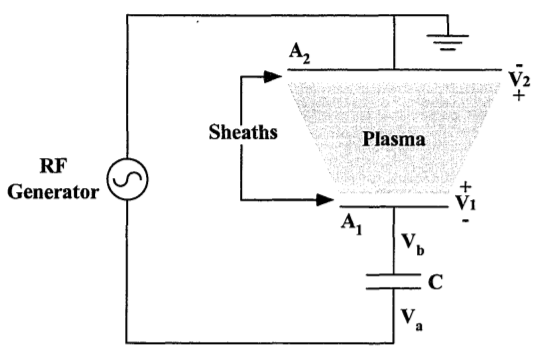
\includegraphics[scale = .75]{Figure 1.5}
	\bf\caption{Schematic of an rf discharge circuit.}
	\label{fig:1.5}
\end{figure}

\begin{figure}[H]
	\centering
	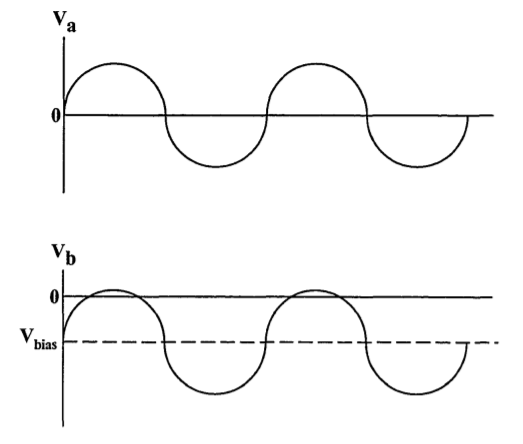
\includegraphics[scale = .75]{Figure 1.6}
	\bf\caption{Voltage waveforms in rf discharge.}
	\label{fig:1.6}
\end{figure}

\noindent atoms than in the bulk; therefore, the sheaths are darker than the rest of the discharge and are also referred to as dark spaces. Complete details of this phenomenon can be found in
[16].

A sheath also develops between the plasma and the grounded electrode leading to a positive plasma potential (V2 ). If it is assumed that the ions traverse the dark space without collision then the voltages between each electrode and the plasma are related by [63]

\begin{align}
	\left( \frac{V_{1}}{V_{2}} \right) &= \left( \frac{A_{2}}{A_{1}} \right) ^{4}
\end{align}

\noindent However, in practice most experiments have shown that

\begin{align}
	\left( \frac{V_{1}}{V_{2}} \right) &\approx \left( \frac{A_{2}}{A_{1}} \right) ^{q}
\end{align}


with q $leq$ 2.5. It is thought that this difference is because the sheaths are not completely collisionless [16]. At process conditions used in this research the mean free path of the ions was on the order of 4 mm and the sheath thickness was measured to be approximately 13 mm. Therefore, ions collide rarely while traversing the dark space and the above relationship approximately holds. In RIE, the chamber walls are part of the grounded electrode; hence, the grounded electrode generally has a much larger surface area than has the powered electrode. This leads to a large bias between the plasma and the powered electrode ($V_{1}$), and a small one with respect to ground ($V_{2}$). The resulting potential distribution is similar to that shown in Figure 1.7. In this figure, the dc bias voltagE refers to the bias of the powered electrode with respect to ground.


\subsection{Etch Mechanisms}

\tab Reactive ion etching is actually a misleading name for the process [21]. A more descriptive name would be ion enhanced etching. In the RIE process, the surface is exposed to both thermal radicals and high energy ions.

\begin{figure}[H]
	\centering
	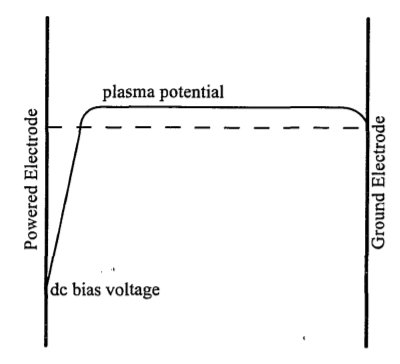
\includegraphics[scale = .6]{Figure 1.7}
	\bf\caption{Potential distribution in an asymmetric parallel plate reactor.}
	\label{fig:1.7}
\end{figure}

\noindent In the case of silicon etching performed in a tetrafluoromethane ($CF_{4}$) plasma, the neutral radicals are fluorine atoms and the ions are mainly $CF^{+}_{3}$. Reactions at the surface lead to the formation of $SiF_{4}$ which desorbs, removing silicon from the surface (Figure 1.8).

\begin{figure}[H]
	\centering
	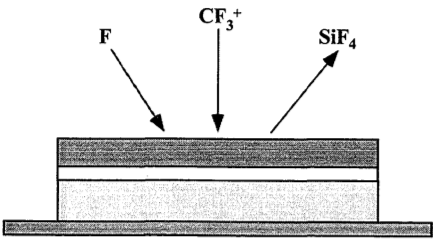
\includegraphics[scale = .6]{Figure 1.8}
	\bf\caption{Etch species and product.}
	\label{fig:1.8}
\end{figure}

\large\bf Role of neutral radicals
\vspace{.5cm}

\normalfont\normalsize A number of steps must occur for etching to take place at the wafer surface. First, the radicals must diffuse to the wafer and adsorb onto the surface. The radicals then react with the surface material to form a volatile reaction product. Etching is complete when these reaction products desorb into the gas phase and diffuse away from the wafer surface. In the case of fluorine etching of silicon, these steps are

\setstretch{1.1}
\begin{align}
	\text{Absorption: }& \text{F}_{gas} \rightarrow \text{F}_{ads}, \\
	\text{Reaction: }& \text{Si}+4\text{F}_{ads} \rightarrow \left( \text{SiF}_{4}\right)_{abs}, \\
	\text{Desorption: }& \left( \text{SiF}_{4}\right)_{abs} \rightarrow \left( \text{SiF}_{4}\right)_{gas},
\end{align}

\noindent where the subscript ÿas denotes species in the gas phase and ads denotes species adsorbed onto the silicon surface. All of these steps are necessary for etching to proceed and any of them can limit the etch rate.

The adsorption step can be rate limited by the supply of fluorine at the surface. Therefore, the flux of fluorine radicals is an important parameter in controlling the etch. In general, the flux of a neutral species is given by [16]


\setstretch{.5}
\begin{align}
	\Gamma_{x} &= \frac{n_{x}\bar{c}_{x}}{4} \text{ per unit area,}
\end{align}

\setstretch{1.5}
\noindent where $n_{x}$ is the concentration and $\bar{c}_{x}$ is the mean speed of species $x$. The mean speed is given by

\setstretch{.4}
\begin{align}
	\bar{c}_{x} &= \left( \frac{8kT}{\pi m_{x}}^{\frac{1}{2}} \right)
\end{align}

\setstretch{1.5}
\noindent where T is the temperature of species $x, m_{x}$, is the mass of species $x$, and $k$ is Boltzmann’s constant. From this equation, it can be seen that the flux of fluorine radicals is proportional to their concentration in the plasma. This fact was important to the development of the control strategy.

\setstretch{1.5}
\noindent\large\bf Role of the Ions

\normalsize\normalfont The role of the ions is not to react with the surface but to enhance reactions involving silicon and fluorine on the surface. In capacitively coupled plasmas, such as those used in reactive ion etching, the etch yield (sihcon atoms etched per incident ion) is typically around 8 [103]. The major etch product is $\text{SiF}_{4}$; therefore, the removal of 8 silicon atoms requires 32 fluorine radicals. This is much more than can be provided by a single $\text{CF}^{+}_{4}$ ion. The main effect of the ions is therefore to enhance the chemical etching process.


There have been several mechanisms proposed to explain the effect of ion bombardment [73]. These include chemically enhanced physical sputtering [75], surface damage enhanced reaction rates [35], and ion assisted gas-surface chemistry. The latter is generally accepted for the case of fluorine etching of silicon [103]. It is believed th at the energy supplied by ions impacting the surface increases the surface mobility, and thus enhances the formation and desorption of volatile products.


Ion bombardment can also change the nature of the reactions on the surface. Molecules of $\text{SiF}_{x}$ will not spontaneously react to form volatile $\text{SiF}_{4}$; thus atomic fluorine is necessary for etching to occur [106]. However, ion bombardment will indeed cause this reaction to occur. In addition, while $\text{SiF}_{2}$ is normally strongly bound to the surface, ion collisions can leave this molecule in a weakly bound state [106]. Hence, the $\text{SiF}_{2}$ can then thermally desorb after the collision.


The degree to which the ions enhance the etch rate is a function of their incident energy. The etch yield for an ion increases with both the ion energy and the flux ratio between,

\setstretch{.75}
\begin{figure}[H]
	\centering
	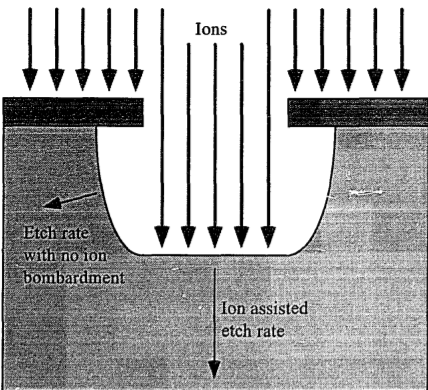
\includegraphics[scale = .5]{Figure 1.9}
	\bf\caption{Directional etch produced by ion bombardment}
	\label{fig:1.9}
\end{figure}

\setstretch{1.5}
\noindent fluorine radicals and ions, approaching saturation for high flux ratios [44]. The removal rate of silicon atoms is thus


\setstretch{.5}
\begin{align}
	\text{Etch Rate} &= p_{0} \left( \frac{\Gamma_{F}}{\Gamma_{Ions}}, \varepsilon_{Ions} \right) \text{ x } \Gamma_{Ions},
\end{align}

\setstretch{1.5}
\noindent where $p_{0}$ is the etch yield, $\Gamma_{F}$ is the flux of fluorine radicals, $\Gamma_{Ions}$ is the flux of ions, and $\varepsilon_{Ions}$ is the energy of the ions. The energy of the ions is given by

\setstretch{1}
\begin{align}
	\varepsilon_{Ions} &= q \left( V_{plasma}-V_{bias}\right),
\end{align}

\setstretch{1.5}
\noindent where $q$ is a unit charge and $V_{plasma}$ is the dc plasma potential shown in Figure 1.7. The plasma potential is generally small {$V_{plasma} \sim 20V$); therefore, assuming that most of the ions are singly charged, $qV_{bias}$ is a good estimate of energy of the ions.
	
In reactive ion etching, it is the enhancement of etch rate due to ion bombardment that causes anisotropic etching. The ions only bombard the surface in areas left unprotected by the mask. Thus, as shown in Figure 1.9, ion enhanced etching occurs on the bottom surface, of a trench, while only
	
\setstretch{1}
	\begin{figure}[H]
		\centering
		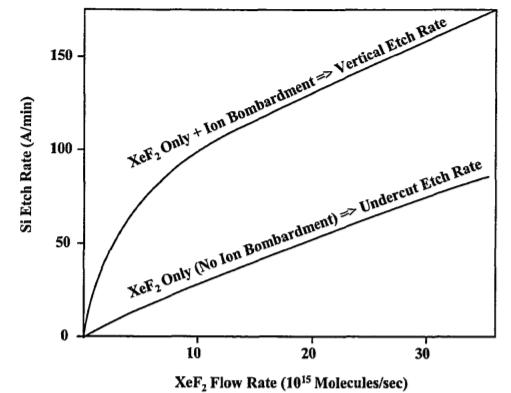
\includegraphics[scale = .6]{Figure 1.10}
		\bf\caption{ Etch rate with and without ion bombardment [38].}
		\label{fig:1.10}
	\end{figure}
	
\setstretch{1.5}
\noindent chemical etching occurs on the sidewalls. The degree of anisotropy is controlled by the flux and energy of the ions, as well as the flux of neutral radicals.
	
\setstretch{.5}
\subsection{Sidewall Passivation}
	
\setstretch{1.5}
\tab Anisotropic etching is important to the production of microelectronic devices with small linewidths. Using ion beam studies with $\text{XeF}_{2}$ gas, it has been shown (see Figure 1.10) that the vertical etch rate and undercut etch rate go to zero together [38]. Therefore, it is not possible to get vertical sidewalls with a fluorine chemistry unless some sort of sidewall passivation is used. One method of achieving vertical sidewalls is by using a chemistry that deposits a polymeric film [42]. In this case, the polymerized films deposit on all the surfaces, including the surfaces of the trench being etched. As shown in Figure 1.11, high directional bombardment by the ions removes this film from the bottom surface but leaves the walls untouched [23]. This continuous clearing of the bottom allows etching to proceed in the
	
	
\setstretch{.75}
	\begin{figure}[H]
		\centering
		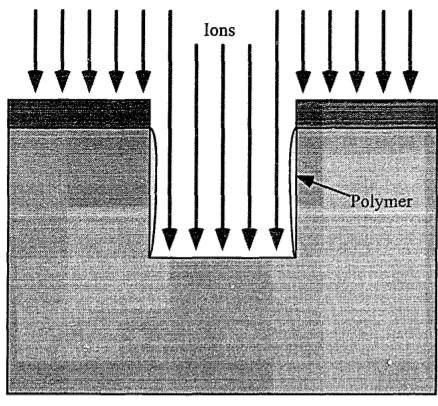
\includegraphics[scale = .6]{Figure 1.11}
		\bf\caption{ Sidewall passivation through polymerization.}
		\label{fig:1.11}
	\end{figure}
	
\setstretch{1.425}
\noindent vertical direction while the polymers inhibit etching of the sidewalls.
	
The key to this technique is to operate the plasma in a regime where polymeric films form on surfaces protected from ion bombardment while etching proceeds on the exposed surfaces. The separation between etching and polymerization can be qualitatively described by the fiuorine-to-carbon (F/C) ratio of the plasma. The ratio includes only those species which participate in the etching or polymerizing chemistry {e.g. $ \text{F}, \text{CF}_{3}, \text{CF}_{2}, \text{CF}, \text{CF}^{+}_{3} $, etc. ) and excludes inert species {e.g. $ \text{CF}_{4}, \text{C}_{2}\text{F}_{6}, \text{SiF}_{4}, \text{CO}, \text{CO}_{2}, \text{HF},$ etc. ). Increasing the ratio leads to increased Si etch rates, and decreasing the ratio lowers the etch rates and encourages polymerization [108]. The threshold between etching and polymerization varies with $\text{V}_{bias}$ as shown in Figure 1.12. The F/C ratio can be varied by the addition of $\text{O}_{2}$ or $\text{H}_{2}$ to the feed gas. The addition of $\text{O}_{2}$ to the plasma chemistry consumes C (by forming CO and $\text{CO}_{2}$), while the addition of $\text{H}_{2}$ consumes F (by forming HF). By controlling the gas chemistry, polymers can be selectively deposited on the sidewalls and thus lead to anisotropic etching.
			
\begin{figure}[H]
	\centering
	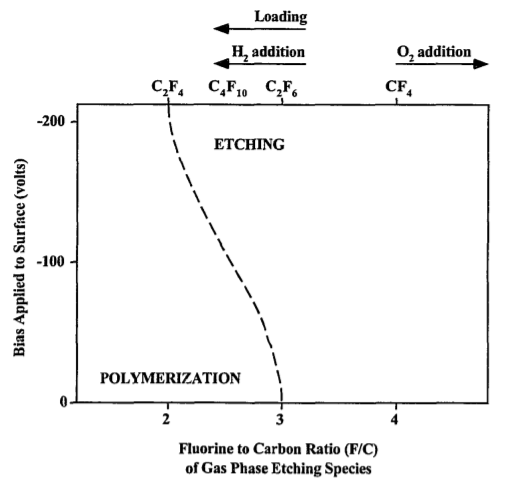
\includegraphics[scale = .6]{Figure 1.12}
	\bf\caption{ Boundary between polymerization and etching as influenced by F /C ratio [23].}
	\label{fig:1.12}
\end{figure}		
			
\section{Applications of Feedback Control to Semiconductor Fabrication Processes}
			
\setstretch{1.5}
\tab Traditional process control in the semiconductor industry has been primarily based on a collection of separate feedback loops relating one measurement of interest to one actuator. Over the past decade, there have been a number of different applications of multivariable feedback control to a variety of fabrication steps. Common to all of these applications is that the control algorithms are based on models of the particular process and in  cases multiple process parameters (either of different process variables or of a single variable at different locations) are controlled by manipulating various equipment parameters. In addition, they all use real-time feedback in the sense that equipment parameters are manipulated during the process to maintain specified process conditions.
			
			
One of the first such applications was undertaken at the University of Texas at Austin. This group explored real-time monitoring and control for reactive ion etching of silicon and silicon dioxide [13,76,77]. This work applied block relative gain array analysis to silicon and silicon dioxide etching with both $\text{CF}_{4}/\text{O}_{2}$ and $\text{CF}_{4}/\text{H}_{2}$ plasmas. It was seen that single loop feedback control was inadequate for both of these etching processes [13]. Multivariable control was found to be effective in reducing dynamic process fluctuations.
			
			
During the fall of 1991, members of the Solid-State Electronics Laboratory and the Control Systems Laboratory at the University of Michigan began joint work on controlling the reactive ion etching process for polysilicon gate etching. An overview of applications of real-time feedback control to RIE at the University of Michigan was presented at the Electrochemical Society’s 187th Meeting [46]. The basic idea of the control strategies is to decompose the reactive ion etching process into a plasma generation process and a wafer etch process. This will be discussed in detail in Section 3.1. Control of plasma characteristics has been shown to reject disturbances to the etch process [29,86,87]. The effect of controlling different sets of plasma characteristics was also explored [30], as well as the benefits of using a multiple-input multiple-output controller versus several “independent” single-input single-output controllers [30,37]. In addition, this control strategy has been applied to etching amorphous silicon for thin film transistors [51]. A similar strategy has been applied to control sidewall profile [85]. The above work has been based on linear models and controllers for the plasma generation process. Nonlinear modeling and control have also been applied [105].
			
Mutsukura, \textit{et. al}. [81] at Tokyo Denki University have applied real-time feedback to control optical sheath thickness and maximum optical intensity in etching plasmas. In this work, the spatial distribution of the optical emission intensity was measured with a CCD camera. Unlike the University of Michigan, no steps were taken to measure any particular wavelength of the emission. Prom this measurement, a sheath thickness and maximum optical intensity were extracted. A real-time feedback controller was used to regulate these plasma parameters by varying chamber pressure and applied power. It was shown that using this technique reduced the variance of etch depth over a number of trials.
			
Another application of modern control techniques has been to Rapid Thermal Processing (RTF) of single wafers. RTF is being explored as a possible way to overcome the uniformity problems associated with multiwafer furnaces [28]. A number of groups have been applying various modeling and control strategies to RTF. A joint group from Stanford University and Texas Instruments’ Microelectronics Manufacturing Science and Technology project have been using low-order nonlinear models of a RTF system [93]. This model was then linearized and its unknown parameters were fit from experimental data [19,95]. Based on this model, feedback control was applied using the Internal Model Control strategy [94]. Likewise, a group from the University of Texas at Austin [28,100] has applied a successively linearized quadratic dynamic matrix control (QDMC) strategy [11] to an RTF developed at Sematech.
			
A strategy similar to that employed at the University of Michigan is being applied to plasma enhanced chemical vapor deposition (FECVD) at Carnegie Mellon University [18,62]. This work has focused on the deposition of silicon nitride using SiIÎ4 and NH3. A quadrapole mass spectrometer is used to measure key partial pressures in the plasma.Experimental results will be presented in the near future [18].
			
All of the applications presented above focus on the processing of silicon wafers. Additionally, real-time control techniques have been applied to the processing of compound semiconductors. Looze, \textit{et al}. [71,72] have applied lead compensation to Czochralski growth of GaAs. Celii, \textit{et al}. [14] have used spectroscopic ellipsometry to control layer thicknesses in AlAs/$\text{In}_{0.53}\text{Ga}_{0.47}$As resonant-tunneling diodes grown using molecular beam epitaxy (MBE).
			
			
\section{Outline of the Dissertation}
			
\tab At the beginning of this introduction, the specific goals of this research were listed. First, it was important to configure our reactive ion etcher to allow the implementation of real-time feedback control. This will be described in Chapter 2. Next, as described in Chapter 3, a control-oriented model of the plasma generation process was developed. This model was used in Chapter 4 to design and implement a controller which rejects etch rate disturbances. The same strategy was employed in Chapter 5 to control sidewall profile. The dissertation will conclude with a discussion of future directions for this research.
			

